% -*-cap2.tex-*-
% Este fichero es parte de la plantilla LaTeX para
% la realización de Proyectos Final de Carrera, protegido
% bajo los términos de la licencia GFDL.
% Para más información, la licencia completa viene incluida en el
% fichero fdl-1.3.tex

% Copyright (C) 2009 Pablo Recio Quijano 

En este capítulo se comentarán las bases del proyecto: fundamentos del dominó y diseño de sistemas expertos.

\section{El dominó}

A continuación se detalla una breve historia del juego del dominó y similares y después se comentan las estrategias fundamentales para jugar el dominó internacional (el que normalmente suele jugarse en España e Iberoamérica).

\subsection{Historia del dominó}

El dominó, deporte y pasatiempo a un tiempo, es un juego que ha ganado adeptos a lo largo de la historia. Según explica \textbf{Miguel Lugo} en su libro Dominó Competitivo \cite{lugo08} éste “es entretenido y fácil de
aprender. Ya desde pequeños comenzamos a jugar al dominó con frutas o con animales en lugar de hacerlo
con puntos”. Además, éste ha ganado popularidad durante los últimos años hasta el punto de televisar
torneos en Europa, Norteamérica y Latinoamérica.

\begin{quote}
“En 2001 la Federación Internacional de Dominó (con sede en Barcelona, España) celebró el primer
Congreso Internacional. El año siguiente se llevó a cabo el primer Campeonato del Mundo de Dominó en La
Habana (Cuba). El ‘Mundial’ continúa celebrándose anualmente a partir de este punto, en España, México,
Venezuela y EEUU" (Lugo, 2008: 1).
\end{quote}

Así pues Lugo señala que el dominó nunca antes ha estado tan reconocido en todo el mundo como ahora, que
incluso se puede jugar por Internet. \\

La página web Dominó en Línea \cite{website:dominoenlinea} recoge que en la actualidad el dominó se juegan en todo el
mundo aunque resalta que es “especialmente popular en América Latina, donde los dominós se consideran
como el juego nacional de numerosos países del Caribe”. Así, también menciona los torneos anuales y
los clubes locales de dominó.

\begin{quote}
El origen del dominó parece ser muy antiguo, al menos en lo que se refiere a juegos similares y quizá
pretéritos al actual” (González Sanz, 2010:22)
\end{quote}

Cuenta \textbf{González Sanz} en su libro El arte del dominó: teoría y práctica \cite{sanz00} que algunos historiadores
creen que puede tener origen chino, ya que éstos jugaban a un juego parecido con impresiones en piedra. Este pudo llegar a Europa a través de mercaderes y viajeros, entre los que se cita al célebre
Marco Polo, los cuales y fruto de los intercambios culturales de la época, trajeron el dominó a este
lado del mundo, más en concreto a la Península Itálica, primer lugar de Europa donde se ha datado la
práctica de este juego. \\

\textbf{Benito Ruipérez} \cite{mora90} también señala que se trata de un juego muy antiguo, de unos 400 años de historia,
aunque dice que se desconoce su origen y etimología (1990:7). Por otro lado, este autor comenta que
llego a Italia desde China en el siglo XVIII, sin embargo, relata que no está probado. “Versiones
coincidentes aseguran que el dominó entró en Europa a través de Italia (con lo que también se puede
atribuir su invención a los italianos, al menos el sistema de juego europeo)”, recoge Ruipérez. \\

Los italianos lo pusieron de moda introduciéndolo en España y Francia a mediados del siglo XVIII,
llegando más tarde a popularizarse de modo extraordinario. A finales del mismo siglo apareció en
Inglaterra, donde fue calificado de ‘juego infantil’, según Ruipérez “nada más lejos de la realidad”.
\textbf{Joseph Strutt} publicó un libro Deportes y Pasatiempos en 1801, en el que, entre otros disparates,
demostró un gran desconocimiento del juego. Así, escribió: “El dominó no tiene mayor interés que
el ponerlo en conocimiento de las personas mayores de este país” (Ruipérez, 1990:7). \\

Precisamente \textbf{Martin Gardner}, experto en juegos, explica que en la literatura occidental no hay
referencias a este juego hasta mediados del siglo XVIII, en que empezaron a jugarse en Italia y
Francia las primeras partidas. Desde ahí, el juego se extendió al resto del continente, y más tarde,
a Inglaterra y América. En Occidente, la colección normal de piezas de dominó ha consistido siempre
en 28 teselas o losetas formadas por dos cuadrados adyacentes, que contienen todos los posibles
pares de dígitos, de 0 hasta 6. \\

\begin{figure}[h]
  \label{Martin_Gardner}
  \begin{center}
    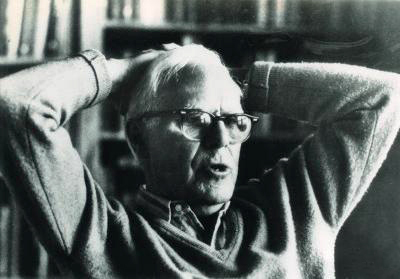
\includegraphics[scale=0.5]{Martin_Gardner.jpeg}
  \end{center}
  \caption{Martin Gardner, divulgador científico y filósofo de la ciencia estadounidense.}
\end{figure}


Respecto al juego chino, Gardner, que colaboró más de 20 años en la sección “Juegos Matemáticos” de
la revista \textbf{Scientific American}, comenta en su libro Circo Matemático que en los dominós chinos,
llamado kwat p’ai, no existen piezas con caras en blanco. Éstos contienen todas las combinaciones
por pares desde el (1-1)  hasta el (6-6), donde tres de los seis puntos de cara son también rojos.
Los dominós coreanos son idénticos, con la única particularidad de que en el as, el punto es mayor
que en las demás piezas. En los dominós chinos, cada pieza tiene un nombre pintoresco: el (6-6)
es el “cielo”; el (1-1) es “la tierra”, el (5-5) es la “flor del ciruelo”, el (6-5), “la cabeza de
tigre”, etc. Los nombres de las piezas son iguales a los que reciben los 21 resultados posibles del
lanzamiento de un par de dados. \\

Ruipérez añade que el invento se les achaca a los chinos “pero no ha de ser muy fiable, ya que el
dominó de chinos y coreanos es muy distinto al que se practica en Europa” (1990:7). Así lo describe
en su Libro del dominó:

\begin{quote}
“El dominó oriental consta de 21 fichas, que representan las permutaciones matemáticas resultantes
de tirar dos dados (cada mitad de una ficha vale por un lado), el ‘uno’ y el ‘cuatro’ son rojos;
además, en los dados chinos intervienen 11 fichas repetidas, con lo que suman un total de 32 fichas
el conjunto de, y para, este juego. Las fichas repetidas se llaman ‘civiles’ y las otras ‘militares’,
distinción importante para ciertos juegos de dominó en China y Corea”.
\end{quote}

González Sanz (2010:22) señala que los dominós chinos “suelen ser en la actualidad de cartón, en vez
de la madera, marfil, pasta, o ébano que es lo habitual en los occidentales, y se manejan como naipes”.
Y al igual que ocurre en Europa y América, con estas piezas se realizan numerosos juegos. Respecto a
los distintos juegos de dominó chinos y coreanos, este autor nos remite a Games of the Orient de Stewart
Culin, obra de 1895 reimpresa en 1958 por Charles Tuttle como la mejor referencia. Asimismo apunta que
no existe un dominó propio en Japón – frente al resto de países asiáticos – y dice que en este país se
juega con el sistema occidental. \\

\begin{figure}[h]
  \label{}
  \begin{center}
    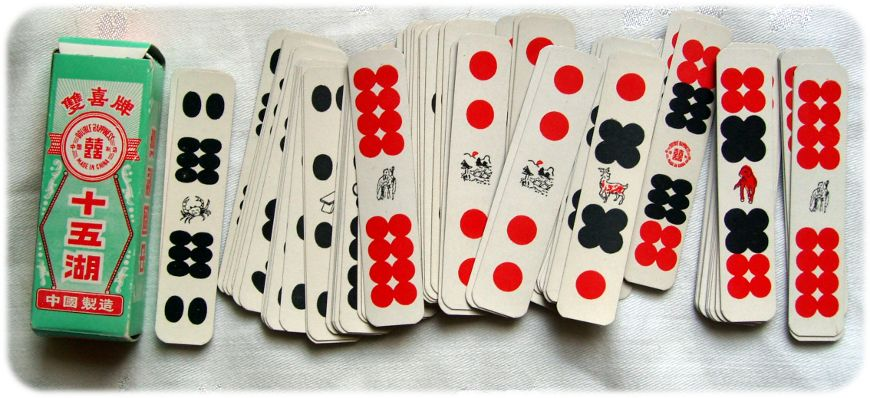
\includegraphics[scale=0.6]{chinese.jpg}
  \end{center}
  \caption{Cartas de dominó chino \textbf{“Double Happiness”} --- los símbolos representan diferentes
            circunstancias y bendiciones de la vida }
\end{figure}

Sin embargo, y aunque por lo que señalan algunos autores el origen asiático del dominó es el más
extendido, también existen otras versiones que atribuyen el invento del juego a árabes o egipcios,
“sosteniendo que no hay pruebas para relacionar claramente el dominó europeo con el chino, pudiendo
ser dos invenciones independientes y separadas en el tiempo” (2010:23). González también cuenta que
se conocen otras versiones del juego como la esquimal o la coreana, con distinto número de fichas
y palos al clásico. \\

Por otro lado, otros autores (desde la página Dominó en Línea \cite{website:dominoenlinea}) apuntan que el dominó
de origen más antiguo se habría encontrado en la tumba de Touthankamon en Egipto. Y que los dominós nacieron de la derivación del juego de dados indio, conocido en Europa bajo el dado a seis-cara, los chinos modificaron este dado en parte plana reversible representando puntos, de 1 en 6 puntos. En Europa sería apareció una cara suplementaria, el blanco. \\

En el apartado de curiosidades que se apunta en esta web podemos destacar que la palabra “dominó”
sería a causa de la semejanza entre las partes de las fichas del juego y la ropa de las religiosas
de las Dominicas (blanco cubierto de un cabo negro). Sin embargo, el autor Ruipérez en el Libro
del Dominó apunta otros posibles orígenes al término, algunos muy parecidos al ya apuntado. De hecho, existe una variante del juego que se juega con fichas de tres caras y se llama \emph{Trimino}, haciendo un juego de do(s)-mino por tri-mino \cite{website:trimino}\\

En este sentido, señala este autor que su nombre se debe, según unos, al revestimiento negro que
llevan sus fichas por el reverso (la espalda), como si fueran cubiertas por un dominó (capuchón
que usaban en el coro, durante el invierno, los monjes). Y según otros, a que tal juego, por su
sencillez, “prueba inequívoca de que no se conocían las técnicas que se usan hoy en día, o de alta
escuela, que son las que se explican en este libro”, estuvo muy en uso en los conventos, y cuando
uno de los jugadores ganaba una partida decía: ‘Benedicamus Dómino’. Una tercera versión para
explicar el nombre afirma que por aquel entonces alguien ya detectó que para ‘manejar’ bien estas
fichas tenía que tener ‘dominio’ de sí mismo (control de lo jugado y de lo pendiente por jugar) en
cada mano, y podría decir, cada vez que querían jugar con estas fichas, ‘vamos a practicar unas
manos al juego del dominio’, habiendo degenerado o perfeccionado el dicho hasta quedar en el juego
del dominó (Ruipérez, 1990:9). \\

En cuanto a la documentación escrita de este juego, este mismo autor,
Ruipérez, señala que el primer libro que hace referencia al juego del
dominó data del año 1786, editado en Amsterdam, según consta en la
Biblioteca Nacional de Bruselas. En total, este autor señala que hay
más de un centenar de libros hasta la fecha (1984), según consta
también en distintas bibliotecas nacionales de Europa y
Latinoamérica. Aunque para este autor no han tenido suficiente éxito
porque no se profundiza en el tema sino que se relatan someramente las
reglas básicas del mismo. En una consulta en la Biblioteca Nacional
aparece como primer libro en español sobre el tema \textbf{Tratado del Juego del Domino, sus Reglas, Combinaciones y Preceptos para ser un buen jugador} de Martínez~\cite{Martinez}, publicado en 1872. \\

En 1982 y después en 1984, más reformado y actualizado, aparece en Barcelona el libro \textbf{ABC del dominó},
de J.M. Vilabella, que denota un conocimiento más amplio del tema comparado con lo que se había
escrito hasta ese momento, dando explicaciones más amplias de cómo se desarrollan las jugadas,
“aunque muy pocas y con muy pocas variantes”, (Ruipérez, 1990:8)

\subsubsection{Tipología de dominós}

Como hemos visto, a lo largo y ancho del mundo existen diferentes tipos de dominó de los que no
siempre los autores coinciden con un solo origen. Aunque para catalogar tales juegos como dominó sí
deben tener una serie de características en común. 

\begin{quote}
Generalizando el concepto de dominó, podríamos decir que es un juego cuyas fichas se encuentran
divididas en dos partes, las cuales señalan mediante incisiones o muescas, un número concreto entre
los posibles palos o números admitidos. Estas fichas contendrán en su totalidad todas las
combinaciones posibles de estos palos, comenzando por la ausencia de puntos o palo de blancos
(González Sanz, 2010:24).
\end{quote}

La Real Academia de la Lengua Española en su primera acepción define este juego como aquel que
“se hace con 28 fichas rectangulares divididas en dos cuadrados, cada uno de los cuales lleva marcados
de uno a seis puntos, o no lleva ninguno. Cada jugador pone por turno una ficha que tenga número
igual en uno de sus cuadrados al de cualquiera de los dos que están en los extremos de la línea de
las ya jugadas, y gana quien primero coloca todas las suyas o quien se quede con menos puntos, si
se cierra el juego”. De este modo, la RAE acota algo más el término acercándose a lo que conocemos
como dominó occidental. \\

\begin{figure}[h]
  \label{Dominoes}
  \begin{center}
    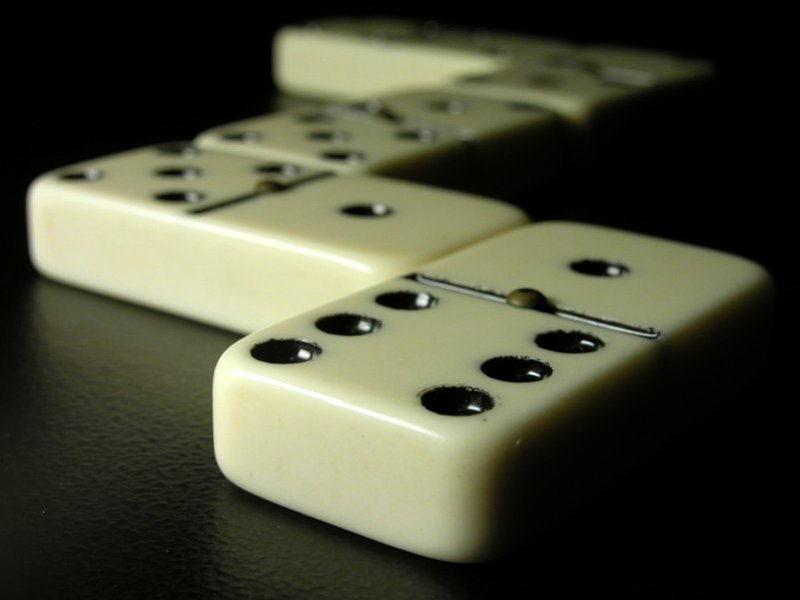
\includegraphics[scale=0.3]{Dominoes.jpg}
  \end{center}
  \caption{Fichas de dominó europeo}
\end{figure}

Según la página Dominó en Línea \cite{website:dominoenlinea} “los dominós son de simples bloques de construcción
que pueden armarse de innombrables maneras con el fin de crear una gran variedad de juegos. Es un
juego que exige mucha capacidad y de estrategia”. \\

Ruipérez define el domino europeo en “un conjunto de veintiocho fichas, por lo general negras y
totalmente lisas por un lado, el reverso o la espalda, y por el otro lado, el anverso o la cara,
divididas en dos mitades con fondo blanco y señaladas con agujeros o puntitos negros; en el centro
de la cara llevan un tornillito con cabeza redondeada, que es el que apoya en la mesa y facilita
el movimiento de las fichas cuando éstas han de ser movidas (barajadas), para que los participantes
cojan sus fichas e inicien la jugada o la mano correspondiente. Tiene siete fichas denominadas
dobles, por en sus medias partes de la cara la misma cantidad de puntitos, a excepción de la
doble blanca, que no lleva ninguno”. \\

\subsection{Reglas básicas}

Aunque las reglas del dominó son sencillas y conocidas por un gran conjunto de lectores, daremos una
serie de pinceladas rápidas sobre las reglas más básicas, siempre recordando que estamos desarrollando
una partida de dominó siguiendo las reglas de la modalidad \emph{Dominó Internacional}. \\

El objetivo del juego es alcanzar una determinada puntuación previamente fijada, jugando para ello las
manos o rondas que sean precisas. En el caso del Dominó Internacional, el número de puntos son 200. En esta modalidad se enfrentan dos equipos, cada uno formado por una pareja de jugadores dispuestos en la mesa de forma alternativa. \\

Antes de empezar, las fichas se colocan boca abajo sobre la mesa y se revuelven para que los jugadores
las recojan al azar en igual número cada uno. Cada jugador cogerá 7 fichas. La primera ronda la comenzará
el jugador que posea el seis doble. En las siguientes rondas, empezará el jugador a la derecha del que
empezó la ronda anterior. Podrá comenzar usando cualquier ficha, no tiene porqué ser doble. \\

En su turno cada jugador colocará una de sus piezas con la restricción de que dos piezas sólo pueden
colocarse juntas cuando los cuadrados adyacentes sean del mismo valor. Si un jugador no puede colocar
ninguna ficha en su turno tendrá que pasar el turno al siguiente jugador. \\

La mano continúa hasta que se da alguna de las dos situaciones:
\begin{itemize}
    \item Alguno de los jugadores se queda sin fichas por colocar en la mesa. En este caso el jugador se
        dice que dominó la partida y la pareja ganadora sumará la totalidad de los puntos no jugados,
        es decir, la suma de los puntos en las fichas que resten por jugar a ambas parejas.
    \item En caso de cierre --- es decir, cuando a pesar de quedar fichas en juego ninguna pueda colocarse ---
        ganará la pareja cuyas fichas sumen menos puntos. Esta situación solamente ocurre cuando el mismo número
        está en ambos extremos del juego, y las siete fichas de ese número ya han sido jugadas. En este caso
        gana la pareja/jugador que menos puntos tenga en sus fichas, y se le suman los puntos del perdedor al ganador.
        Al igual que en el anterior caso, la pareja ganadora sumará la totalidad de los puntos no jugados,
        es decir, la suma de todos los puntos en las fichas que resten por jugar a ambos equipos.
\end{itemize}

\begin{figure}[h]
  \label{cierre}
  \begin{center}
    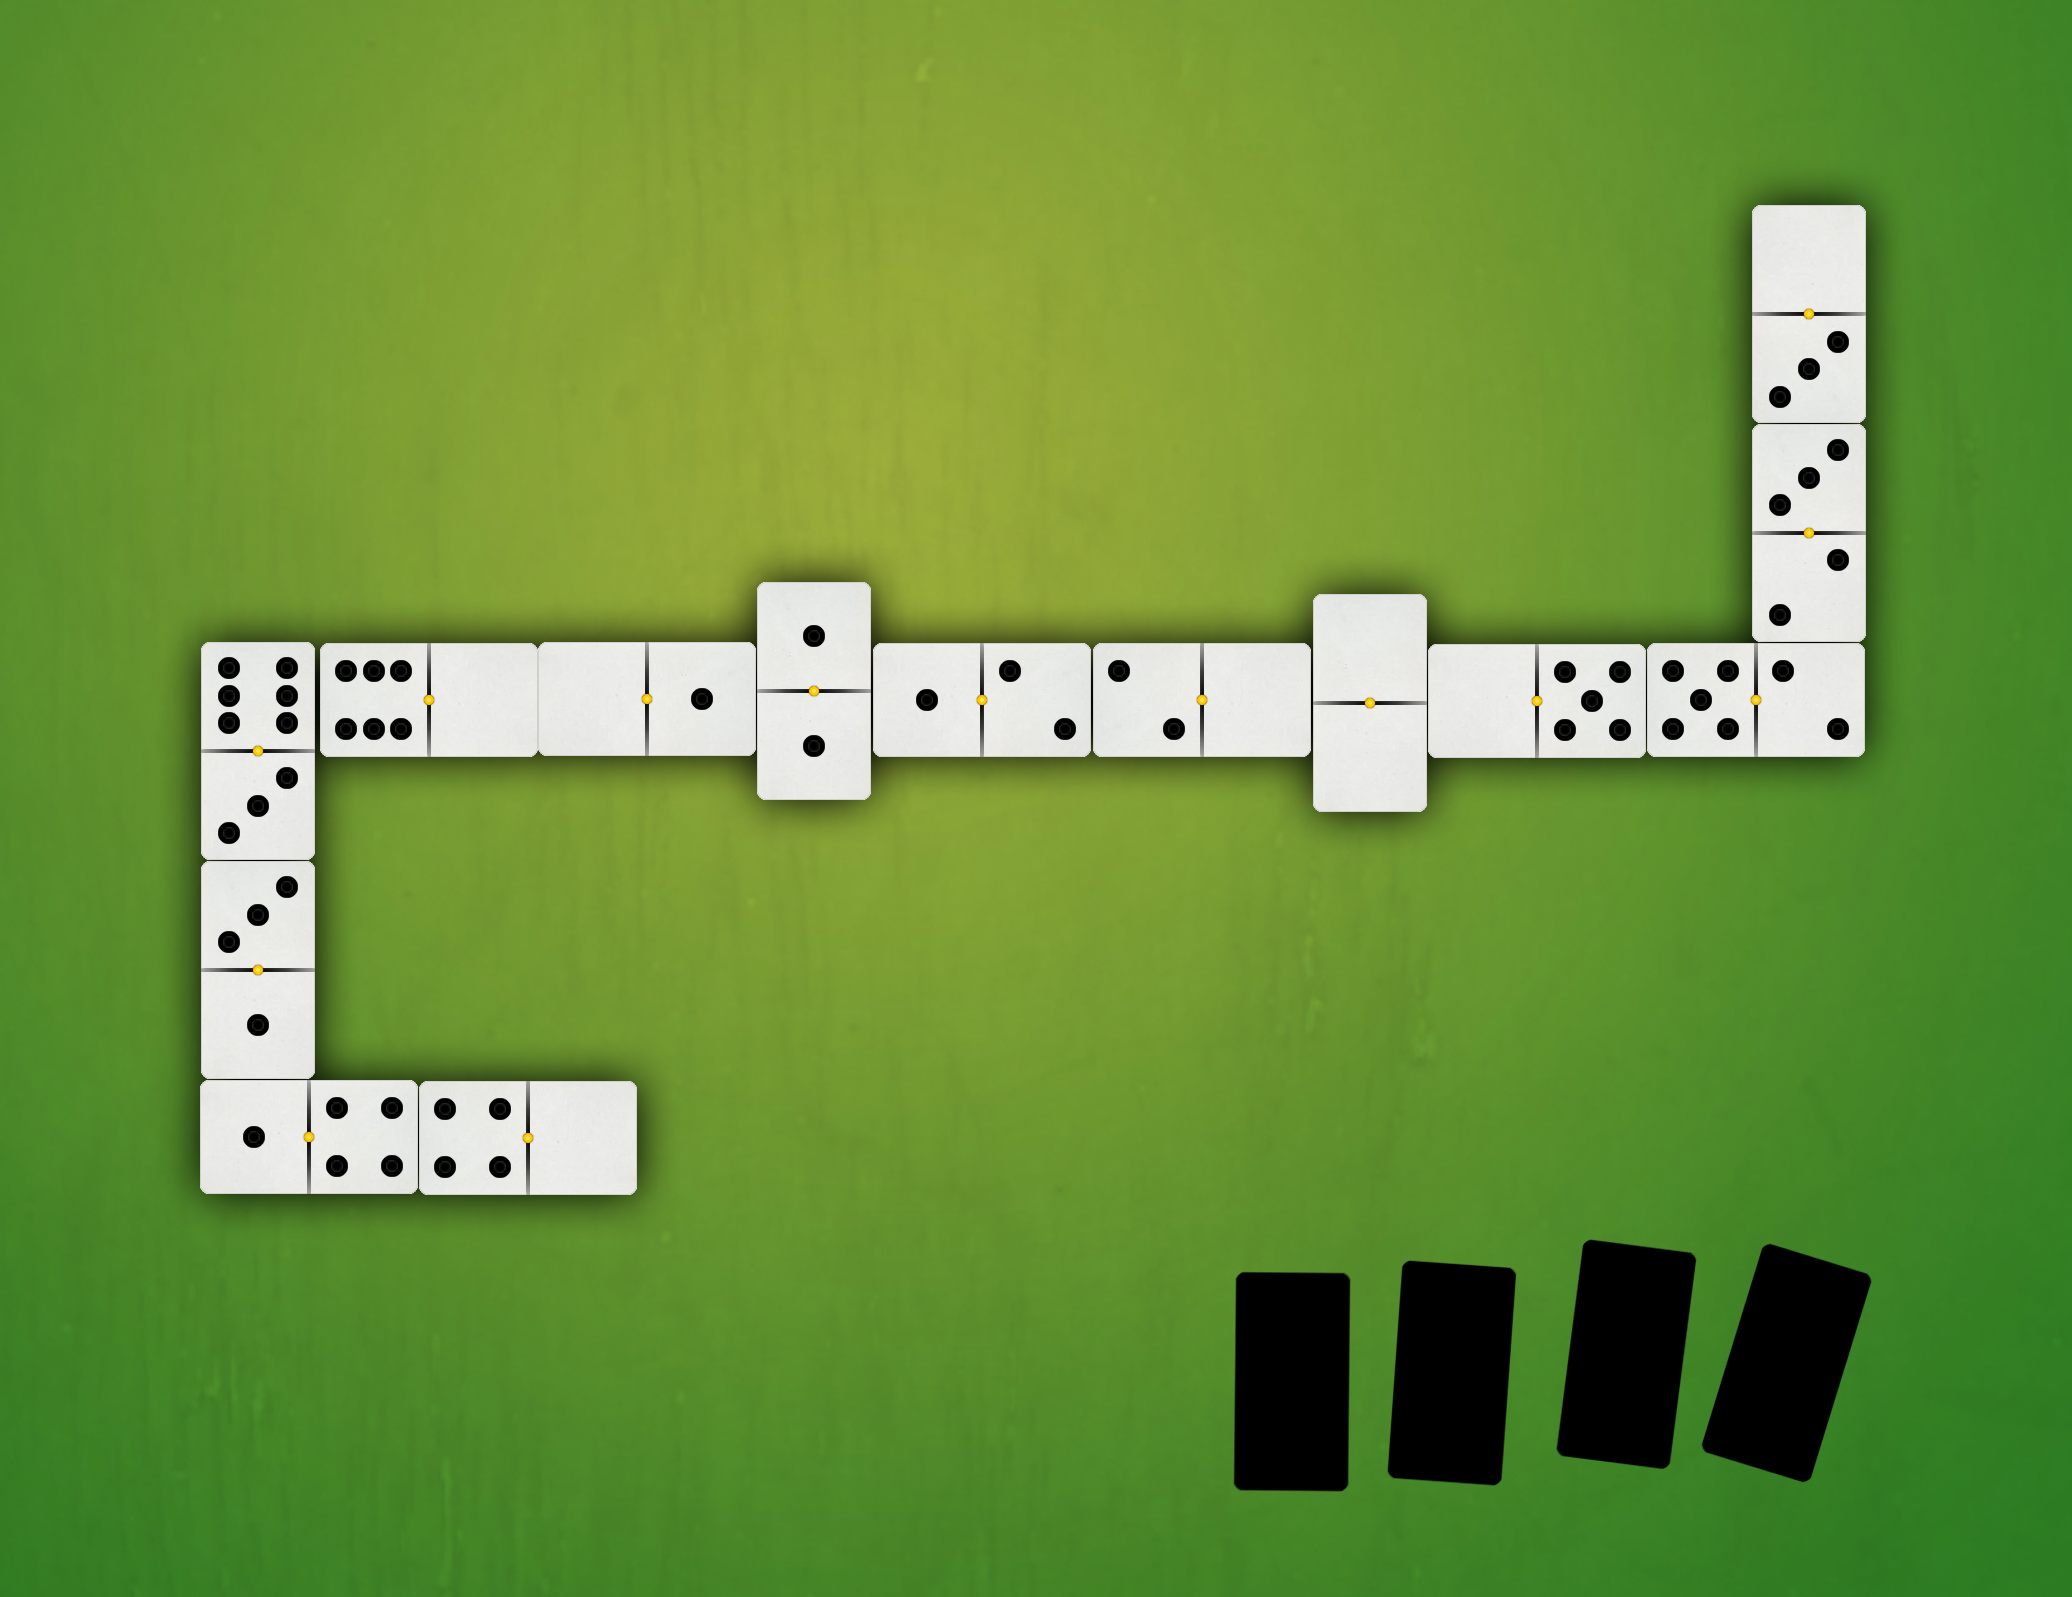
\includegraphics[scale=0.2]{cierre.png}
  \end{center}
  \caption{Ejemplo de partida terminada en cierre. Se han colocado todas las blancas, por lo que no es posible
            que algún jugador continúe la partida}
\end{figure}


La partida finaliza una vez que un equipo ha alcanzado o superado los 200 puntos. \\

\subsection{El dominó es un juego de señores}

Una gran frase que resume la filosofía del Dominó es que \emph{el dominó es un juego de señores}. Esta frase
viene a describir tanto la filosofía del juego como parte de las reglas que lo normalizan, y tendrá mucha
repercusión en cuanto al diseño del sistema experto, por lo que que pasamos a explicarla a continuación. \\

Durante el transcurso de una partida de dominó las parejas no pueden comunicar ningún tipo de información
que pueda afectar al desarrollo normal de la partida, estando totalmente prohibidos cualquier tipo de gestos
entre jugadores destinados a comunicar futuras intenciones, fichas o estrategias conjuntas. Pero existe
una excepción a esta regla. \\

La única seña o gesto válido en el juego del dominó es \emph{la pensada}. Cuando toca el turno de jugar, se tiene la
opción de pensar durante un tiempo relativamente largo para hacerle entender al compañero que se tienen
varias fichas del mismo número que va a tapar o que va a cuadrar. O por el contrario, jugar de inmediato,
sin pensar, indica que no se tienen más fichas de ese número. \\

Por lo tanto, a la hora de colocar una ficha sobre la mesa podemos --- aunque quizás tendríamos que decir que 
debemos --- comunicar cierto tipo de información a todos los jugadores de la mesa. Esta información resulta
tremendamente valiosa, y puede hacer que la partida se decante sobre un equipo o sobre el otro. \\

Hemos resaltar y aclarar que, como bien dicta la frase de que \emph{el dominó es un juego de señores},
esta seña no puede utilizarse para confundir o engañar al contrario, y en los diferentes torneos o campeonatos
de dominó supone la descalificación inmediata.


\subsection{Juego por parejas}
\label{juegoporparejas}

El juego por parejas que caracteriza el dominó internacional, a diferencia de otros tipos de modalidades,
determina las estrategias que han de seguirse para que un equipo consiga la victoria, ya que esta únicamente
se consigue trabajando en equipo; como juego de mesa por equipos, necesita imprescindible colaboración
mutua entre compañeros si se quiere conseguir la victoria común. \\

En el desarrollo de una partida los jugadores van desempeñando consecutivamente diferentes roles. Para designar
a cada jugador, es común utilizar la siguiente nomenclatura: 

\begin{description}
    \item[j1] Jugador mano que inicia la mano
    \item[j2] Jugador a la derecha del que inicia la partida
    \item[j3] Compañero del jugador que inicia la mano
    \item[j4] Compañero del jugador j2, tiene a su derecha al jugador que inicia la mano.
\end{description}

Desde el punto de vista de un jugador concreto, las posibilidades son: \\
\begin{description}
    \item[Ser el jugador mano --- jugador que inicia la partida] Este jugador es el que debe dominar la mano, ya
        que al comenzar está orientando la partida hacia la posición que le interesa; normalmente, intentará
        que el juego se mueva por el palo del que tenga más fichas. Este jugador también cuenta
        con la ventaja de que, al ser el primero que coloca ficha (salvo que no pueda jugar algún turno), es el que tiene siempre igual o menor número
        de fichas que cualquier otro jugador y puede quedarse sin ninguna antes. \\
        Por estas circunstancias, es el único jugador que puede (y debe) jugar para beneficio propio.
    \item[Segundo jugador --- jugador a la derecha del que inicia la partida] La labor de este jugador es
        evitar que el jugador mano desarrolle su estrategia, \emph{matando} las fichas con las que inicie e intentando
        reorientar la partida hacia una posición más ventajosa para él o para su compañero.
    \item[Tercer jugador --- compañero del jugador mano] Este jugador debe apoyar en la medida de lo posible
        la estrategia del jugador mano. Su juego está supeditado en origen a colocar fichas del palo con el
        que haya comenzado su compañero, con la intención de facilitarle el juego y que pueda dominar a ese palo. 
    \item[Cuarto jugador --- a la izquierda del jugador mano] este jugador debe intentar matar las fichas que coloque
        la pareja del jugador mano, y evitar que el juego se desarrolle por el palo al que abrió el jugador mano.
\end{description}

Más tarde, dependiendo de las circunstancias de la partida, los roles
pueden ir cambiando al no poder jugar algunos jugadores sus turnos. En
todo caso, el jugador referencia será el que tenga menos fichas que el
resto, pues, si no pasara ningún turno, ganaría la partida. Este puede
intentar ganarla por sí mismo si contempla la posibilidad y estima que
sus adversarios están a la espera de sus movimientos.


\subsection{Técnicas avanzadas}

% TODO FIXME

Soltar dobles

Cierres

Salida en falso

Jugar para el otro

Exceso de fichas de un tipo (de un sólo número, dobles, etc).


\section{Inteligencia artificial}

A la hora de afrontar un proyecto que simule cierto comportamiento \emph{humano}, debemos usar técnicas de Inteligencia Artificial, en busca de herramientas y metodologías que nos ayuden a afrontar este difícil problema, probablemente uno de los más complicados dentro de la Ingeniería Informática. 

\subsection{Sistemas expertos}

Para implementar la inteligencia de los contrincantes de Dominous se utilizará un
\textbf{sistema experto}~\cite{Giarratano:1989:ESP:583478}.
El desarrollo de sistemas expertos es una rama de la Inteligencia Artificial, que imita los mecanismos y la forma de
pensar de un experto en cierta materia para resolver problemas de su campo de aplicación. Esto lo hace adecuado ara un juego como el dominó, cuyas estrategias ganadoras son conocidas. Estos sistemas tiene un gran implantación en diversas ramas de la ciencia, como medicina, ingeniería o sistemas de decisiones para negocios.\\

\subsubsection{Arquitectura general}

Si consideramos el sistema una caja negra, el usuario del sistema experto sólo tiene que proporcionarle información sobre el problema y recibirá como respuesta el consejo del sistema. Para ello el sistema incorpora internamente dos elementos: la base de conocimiento (donde se almacena la información conocida) y el motor de inferencia (que permite obtener las respuestas adecuadas a partir de la información que el usuario introdujo y la base de conocimiento). La figura~\ref{fig:sistexp} muestra esta arquitectura. \\

\begin{figure}[h]
  \begin{center}
    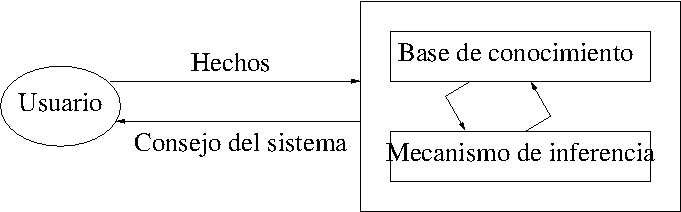
\includegraphics[scale=1]{sistexp.png}
  \end{center}
  \caption{Esquema conceptual de un sistema experto}
  \label{fig:sistexp}
\end{figure}

\subsubsection{Desarrollo de un sistema experto}

El proceso de construcción de un sistema experto se denomina ingeniería del conocimiento. Se basa en una serie de fases que se iteran hasta conseguir un sistema adecuado (figura~\vref{fig:des_sistexp}). En una primera etapa el ingeniero de conocimiento tiene una entrevista con el experto, del que intenta obtener sus conocimientos. Después los implementa en el sistema. Y, por último, el experto evalúa el sistema. Si la evaluación no es del todo satisfactoria, se repite el proceso para refinar el resultado. \\

\begin{figure}[h]
  \begin{center}
    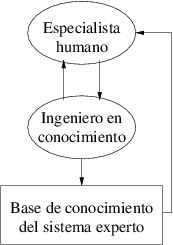
\includegraphics[scale=1.2]{des_sistexp.png}
  \end{center}
  \caption{Desarrollo de un sistema experto}
  \label{fig:des_sistexp}
\end{figure}


\subsection{Sistemas expertos basados en reglas}

De los diversos tipos de sistemas expertos que existen~\cite{ShuHsienLiao200593} este trabajo se centrará en los sistemas expertos basados en reglas. Estos son los más adecuados para un simulador de dominó al ser este un problema con conocimiento parcial del entorno (esto es, se saben las fichas que hay en la partida, pero no qué jugador tiene cada una de ellas) y cuya inteligencia está bien estudiada y expresada en reglas concretas~\cite{Borrajo1990129}. Aún así, existe en la bibliografía una aproximación basada en redes bayesianas~\cite{PFCRoss}. \\

No este el primer trabajo en este sentido, pues existen diferentes aplicaciones de los sistemas expertos basados en reglas a todo tipos de juegos, desde sistemas en tiempo real~\cite{DBLP:conf/robocup/FathzadehMMS05} a diversos juegos de tablero (como~\cite{PFCRecio} o~\cite{PFCChaves}). \\

Los sistemas expertos basados en reglas (sistemas expertos a secas a partir de
ahora) suelen estar dividido en seis partes principales, como se
observa en la figura \ref{fig:arq_sistexp_reg}. A continuación se
detallan cada una de ellas.

\begin{figure}[h]
  \begin{center}
    \resizebox{0,8\linewidth}{!}{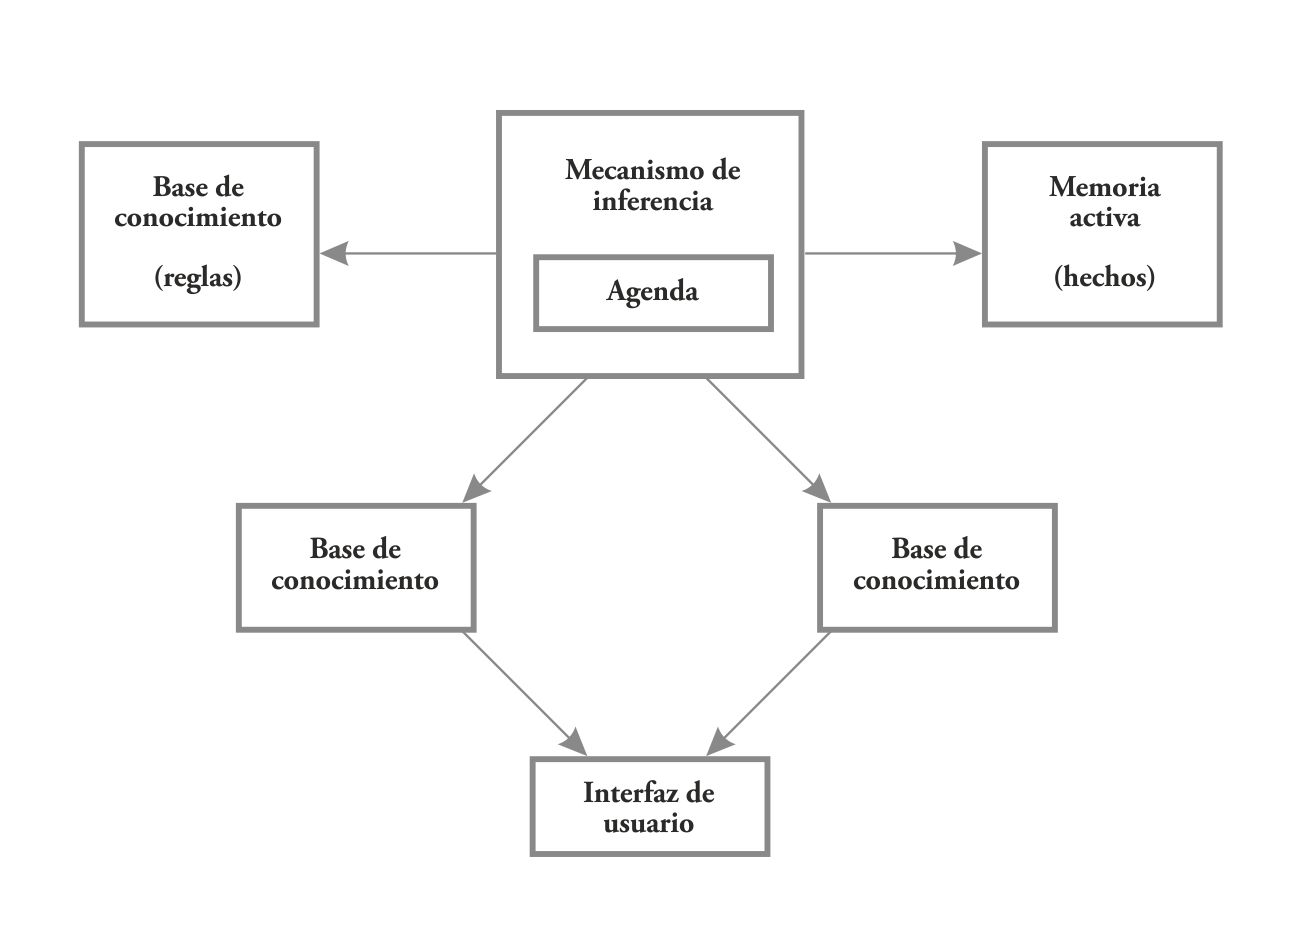
\includegraphics{arq_sistexp_reg.png}}
  \end{center}
  \caption{Arquitectura general de un sistema experto basado en reglas.}
  \label{fig:arq_sistexp_reg}
\end{figure}

\begin{description}
    \item[Base de conocimiento] Contiene conocimiento extraído del experto en forma de reglas.
    \item[Base de hechos (o Memoria activa de trabajo)] Contiene los hechos sobre un problema que se conocen.
    \item[Mecanismo de inferencia] Motor que implementa el proceso de
      razonamiento humano. Comprueba las reglas que satisface la
      memoria activa y ejecuta la que corresponda. Incluye la Agenda,
      que es el conjunto de reglas satisfechas en un momento dado.
    \item[Módulo de justificación (o Medio de explicación)] Detalla el razonamiento utilizado por
      el sistema para llegar a la conclusión proporcionada al usuario.
    \item[Medio para la adquisición de conocimiento] Permite al
      usuario introducir nuevo conocimiento en el sistema sin tener
      que mediar el ingeniero de conocimiento. El sistema suele
      recibir ejemplos para aprender de ellos.
    \item[Interfaz de usuario] Implementa la interacción del usuario con
      el sistema. La interacción la puede realizar tanto una persona
      como otro sistema que desee hacer uso del sistema experto.
\end{description}

En los siguientes apartados se desarrollan los elementos más
importantes: la memoria activa, la base de conocimiento y el motor de
inferencia.

\subsubsection{Memoria activa}

Mantiene una base de datos con la información del sistema. Esta
varía constantemente, tanto por información que se reciba
del exterior (del problema, en general) como por la información
interna que modifiquen las reglas de la base de conocimiento. \\

Está formada por dos tipos de elementos: las plantillas y los
objetos. Las plantillas definen la estructura de la información que se
almacena. En concreto especifican los atributos (del inglés
\emph{slots}) que podrán tener los objetos. Y los objetos en sí
almacenan información de acuerdo a la estructura indicada en las
plantillas.


\subsubsection{Base de conocimiento}

La base de conocimiento (también llamada \emph{sistema de producción}) de un
sistema experto es el conjunto formado por todo el conocimiento que
tiene el sistema en un momento dado. Existen sistemas en los que el
conocimiento se mantiene constante a través del tiempo (la mayoría), y
otros en los que el sistema aprende conocimiento a lo largo de su
vida. \\

El conocimiento se almacena en forma de reglas. Las reglas suelen
estar almacenadas como expresiones ``Si CONDICIÓN entonces
ACCIÓN''. Un ejemplo sería:

\begin{lstlisting}[caption={Regla en pseudocódigo}, numbers=left]
  (defrule biblioteca-regla-1
    (libro (titulo ?X) (estado retraso) (prestado-a ?Y))
    (persona (nombre ?Y) (domicilio ?Z))
    =>
    (mandar-nota-retraso ?X ?Y ?Z))
\end{lstlisting}

Esta regla en lenguaje natural se podría leer línea a línea:
\begin{lstlisting}[caption={Regla en lenguaje natural}, numbers=left]
Regla 1:
  Si
    hay un libro, titulado X, con retraso, y 
    prestado a una persona de nombre Y
    Y
    el domicilio de la persona Y es Z
  Entonces
    mandarle una nota de retraso a Y en Z del libro X
\end{lstlisting}

El libro y persona en concreto deben de estar en la memoria activa. Y
las acciones (como ``mandar-nota-retraso'' del ejemplo) se definen en
funciones escritas por el usuario. \\

En la bibliografía se suele denominar antecedente (o parte izquierda
de la regla\footnote{En inglés \emph{Left-Hand-Side}
  (\emph{L.H.S.}).}) a la condición que tiene el ``Si'', y
consecuente (o parte derecha de la regla \footnote{En inglés
  \emph{Right-Hand-Side} (\emph{R.H.S.}).}) a su acción. \\


\subsubsection{Motor de inferencia}

Su cometido es aplicar el conjunto de reglas del tipo ``si-entonces''
de la base de conocimiento al conjunto de datos que están en la
memoria activa en un momento dado. \\

La \emph{agenda} es el conjunto de reglas que se pueden ejecutar en un
momento del tiempo dado. Hay que tener en cuenta que no es lo mismo la
activación que la ejecución de una regla. La activación indica que la
regla se puede disparar (porque se satisface su condición en el
``Si''). Pero en un instante del tiempo puede haber más más de una
regla activa. Y si una de ellas se ejecuta (se dispara) puede provocar
cambios en la memoria activa e introducir o eliminar reglas de la
agenda. Además hay que tener en cuenta que en algunos sistema (sobre
todo en sistemas en tiempo real) la memoria activa puede estar
recibiendo información constantemente, lo que provoca muchas
modificaciones en la agenda tras disparar una regla y actualizar la información del mundo real. \\

En concreto, el método seguido para determinar qué regla de la agenda
se dispara se denomina \emph{estrategia de resolución de
  conflictos}. Existen muchas de ellas, que pueden ser combinadas:
asignando prioridades a las reglas, disparar primero las reglas menos
usadas (o más las usadas), disparar las reglas con mayor (o menor)
número de condiciones, etc. \\

El algoritmo más simple para implementar el motor de inferencia
(llamado \emph{regla de aproximación a la búsqueda de hechos}) sería
recorrer circularmente de modo indefinido el conjunto de reglas,
buscando reglas que se satisfagan y ejecutándolas. El problema es que
tiene una complejidad computacional de orden $O(R*F^P)$, siendo
\emph{R} el número de reglas, \emph{P} la media de comprobaciones por
el \emph{L.H.S.} de cada regla y \emph{F} la cantidad de reglas de la
base de conocimiento. Evidentemente, este orden no es deseable para
sistemas grandes, pues se dispara al incrementarse las comprobaciones
por regla, por lo que pueden necesitarse optimizaciones~\cite{springerlink:10.1007/1155698575}. Sin embargo, como veremos, es suficiente para problemas
pequeños como puede ser jugar una partida de dominó.



